\documentclass{article}
\usepackage[light, inline-math]{chs-physics-report}
\usepackage{float}
\usepackage{pgfplots}
\usepackage{pgfplotstable}
\usepackage{booktabs}
\graphicspath{{./images/}}

\pgfplotsset{compat=1.18}

\title{11.2: DC Circuits Lab}
\name{Gavin Chen}
\ww{Daniel Aronov}

\begin{document}
\section{Series}
\subsection{Circuit}
\begin{center}
    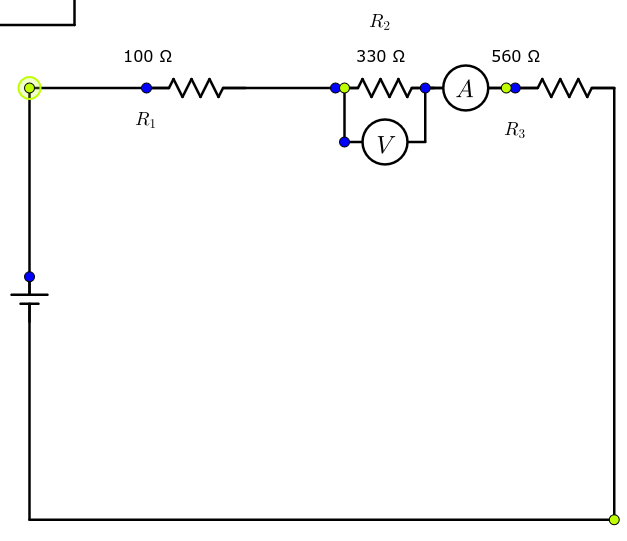
\includegraphics[scale=0.5]{series}
\end{center}
\subsection{Data}
\subsubsection{Theoretical}
\begin{figure}[H]
    \begin{center}
        \pgfplotstabletypeset[col sep=comma, /pgf/number format/fixed, fixed zerofill, precision=4, every head row/.style={
                    before row={
                            \toprule
                        },
                    after row={
                            \bottomrule
                        },
                },
            every last row/.style={
                    after row=\bottomrule
                }]{Series Theoretical.csv}
        \caption{Resistor 0 is the complete circuit with all three resistors.}
    \end{center}
\end{figure}
\subsubsection{Measured}
\begin{figure}[H]
    \begin{center}
        \pgfplotstabletypeset[col sep=comma, /pgf/number format/fixed, fixed zerofill, precision=4, every head row/.style={
                    before row={
                            \toprule
                        },
                    after row={
                            \bottomrule
                        },
                },
            every last row/.style={
                    after row=\bottomrule
                }]{Series Measured.csv}
        \caption{Resistor 0 is the complete circuit with all three resistors.}
    \end{center}
\end{figure}
\subsection{Questions}
\begin{enumerate}
    \item The experimental results agree with the theory, where the total resistance of resistors in series is the sum of the resistance of each individual resistor and current through resistors in series stays constant while voltage drops in between each resistor.
    \item Our experimental results are very close to our theoretical results, with a very small amount of difference between them.
\end{enumerate}

\section{Parallel}
\subsection{Circuit}
\begin{center}
    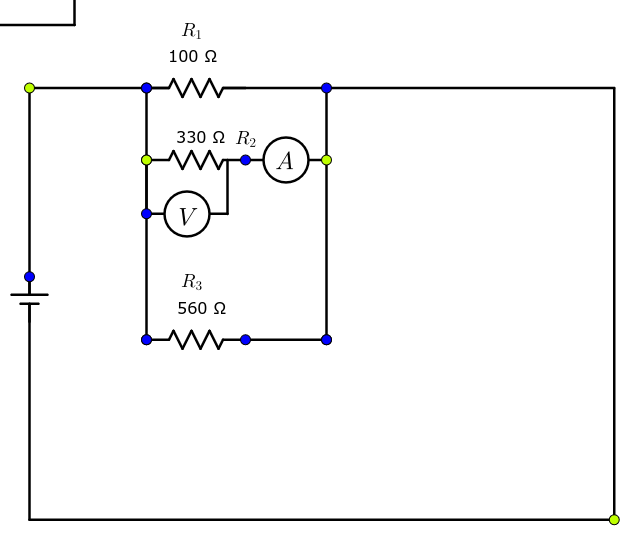
\includegraphics[scale=0.5]{parallel}
\end{center}
\subsection{Data}
\subsubsection{Theoretical}
\begin{figure}[H]
    \begin{center}
        \pgfplotstabletypeset[col sep=comma, /pgf/number format/fixed, fixed zerofill, precision=4, every head row/.style={
                    before row={
                            \toprule
                        },
                    after row={
                            \bottomrule
                        },
                },
            every last row/.style={
                    after row=\bottomrule
                }]{Parallel Theoretical.csv}
        \caption{Resistor 0 is the complete circuit with all three resistors.}
    \end{center}
\end{figure}
\subsubsection{Measured}
\begin{figure}[H]
    \begin{center}
        \pgfplotstabletypeset[col sep=comma, /pgf/number format/fixed, fixed zerofill, precision=4, every head row/.style={
                    before row={
                            \toprule
                        },
                    after row={
                            \bottomrule
                        },
                },
            every last row/.style={
                    after row=\bottomrule
                }]{Parallel Measured.csv}
        \caption{Resistor 0 is the complete circuit with all three resistors.}
    \end{center}
\end{figure}
\subsection{Questions}
\begin{enumerate}
    \item The experimental results agree with the theory, where the total resistance of resistors in parallel is the reciprocal of the sum of the reciprocals of the resistances of each indivudual resistor and voltage through resistors in parallel stays constant while current drops in between each resistor.
    \item Our experimental results are very close to our theoretical results, with a very small amount of difference between them.
\end{enumerate}

\section{Combo}
\subsection{Circuit}
\begin{center}
    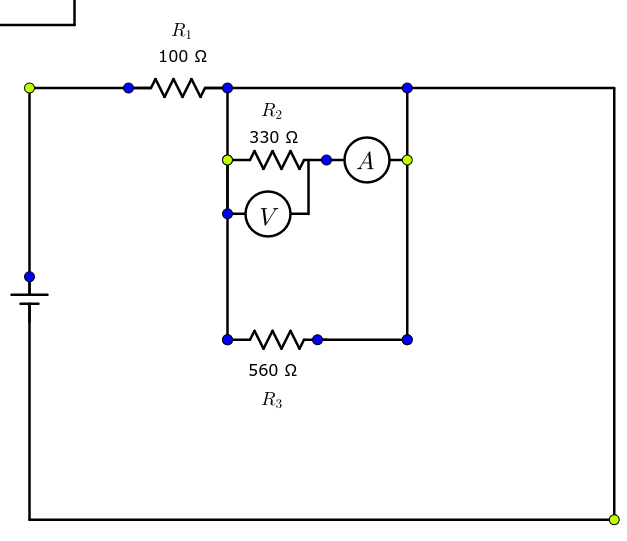
\includegraphics[scale=0.5]{combo}
\end{center}
\subsection{Data}
\subsubsection{Theoretical}
\begin{figure}[H]
    \begin{center}
        \pgfplotstabletypeset[col sep=comma, /pgf/number format/fixed, fixed zerofill, precision=4, every head row/.style={
                    before row={
                            \toprule
                        },
                    after row={
                            \bottomrule
                        },
                },
            every last row/.style={
                    after row=\bottomrule
                }]{Combo Theoretical.csv}
        \caption{Resistor 0 is the complete circuit with all three resistors.}
    \end{center}
\end{figure}
\subsubsection{Measured}
\begin{figure}[H]
    \begin{center}
        \pgfplotstabletypeset[col sep=comma, /pgf/number format/fixed, fixed zerofill, precision=4, every head row/.style={
                    before row={
                            \toprule
                        },
                    after row={
                            \bottomrule
                        },
                },
            every last row/.style={
                    after row=\bottomrule
                }]{Combo Measured.csv}
        \caption{Resistor 0 is the complete circuit with all three resistors.}
    \end{center}
\end{figure}
\subsection{Questions}
\begin{enumerate}
    \item The experimental results agree with the theory, which is a combination of both the series and parallel theories mentioned above.
    \item Our experimental results are very close to our theoretical results, with a very small amount of difference between them.
\end{enumerate}
\end{document}